\tikzset{>=stealth',shorten >=1pt,
  computer node/.style={
        rectangle, align=center,
        minimum width=1.4cm,minimum height=1.3cm,draw,
        append after command={
        \pgfextra
        \draw node[draw,minimum width=1.2cm,minimum height=1.1cm] at (\tikzlastnode.center) {};
        \draw node[draw,minimum width=1.5cm,minimum height=0.6cm] at ([yshift=-0.4cm]\tikzlastnode.south) {};
        \draw node[circle, fill=black, minimum size=0.15cm, inner sep=0pt] at ([xshift=0.55cm,yshift=-0.25cm]\tikzlastnode.south) {};
        \endpgfextra
      }
  }
}
\newsavebox{\documentt}
\savebox{\documentt}{
  \begin{tikzpicture}
    \draw (3,4) -- (3,2.75) to[out=-100,in=100] (5,2.75) -- (5,4) -- (3,4);
    % \draw (0,0) -- (1,-0.1666666);
    % \draw (-1.2,0.2) -- (-2.2,0.366666);
    % \draw (-1,0) -- (-2,-0.1666666);
    % \draw (-0.2,0.2) -- (0.8,0.366666);
  \end{tikzpicture}
}


\newsavebox{\cubesatbox}
\savebox{\cubesatbox}{
  \begin{tikzpicture}
    \draw (0,0) rectangle(-1,-1)
    -- (-1.2,-0.8) -- (-1.2,0.2) -- (-1,0) -- (-1.2,0.2)
    -- (-0.2,0.2) -- (0,0);
    \draw (0,0) -- (1,-0.1666666);
    \draw (-1.2,0.2) -- (-2.2,0.366666);
    \draw (-1,0) -- (-2,-0.1666666);
    \draw (-0.2,0.2) -- (0.8,0.366666);
  \end{tikzpicture}
}

\newcommand{\documentTikz}[1]{\scalebox{#1}{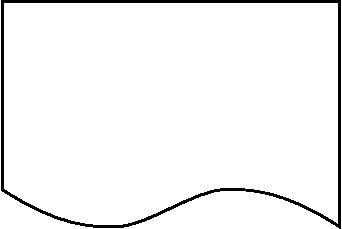
\includegraphics{styles/document.pdf}}}
